%%%%%%%%%%%%%%%%%%%%%%%%%%%%%%%%%%%%%%%%%
% Proyecto Especial de Grado para UC Ing. en Telecomunicaciones 
% Plantilla LaTeX
% Version 1.4 (28/11/15)
%
% Esta plantilla fue descargada desde:
% http://www.latextemplates.com
%
% Autores Originales:
% Steven Gunn 
% http://users.ecs.soton.ac.uk/srg/softwaretools/document/templates/
% y
% Sunil Patel
% http://www.sunilpatel.co.uk/thesis-template/
%
% Modificaciones, Adaptaciones y Traducción:
% Carlos Mejías
% Ahmad Osman
%
%
% Licencia:
% CC BY-NC-SA 3.0 (http://creativecommons.org/licenses/by-nc-sa/3.0/)
%
%%%%%%%%%%%%%%%%%%%%%%%%%%%%%%%%%%%%%%%%%

%----------------------------------------------------------------------------------------
%	PAQUETES Y OTRAS CONFIGURACIONES DEL DOCUMENTO
%----------------------------------------------------------------------------------------

\documentclass[11pt,twoside]{Project} % Tamaño de la fuente, tamaño de la hoja con opción doble cara.

\graphicspath{{Figuras/}} % Especificación del directorio donde se encuentran almacenadas las imágenes

\title{\ttitle} % Define el título del Proyecto Especial de Grado - NO MODIFICAR.

\begin {document}

\renewcommand{\thelstlisting}{\arabic{chapter}.\arabic{lstlisting}} % Define el formato del caption de los códigos. - NO MODIFICAR -

\frontmatter % Numeración romana (i, ii, iii, iv...) para las páginas de pre-contenido. NO MODIFICAR
%
\setstretch{1.4} % Interlineado - NO MODIFICAR

%----------------------------------------------------------------------------------------
%	VARIABLES DEL DOCUMENTO
%----------------------------------------------------------------------------------------

\titulo{Título del Proyecto Especial de Grado} % Título de su Proyecto Especial de Grado. Este título se utiliza tambien en el resumen
%-------------------------------------------------  
\tutor{Nombre del Tutor} % Nombre del tutor - Utilizado en una de las portadas y resumen
%-------------------------------------------------   
% En caso de que sea un sólo autor comente los comandos \autorII, \cedulaII y \tlfII
%-------------------------------------------------
\autorI{Nombre del Autor 1}  % Nombre del 1er autor
\cedulaI{11.111.111}         % C.I del 1er autor
\tlfI{5555-5555555}
\autorII{Nombre del Autor 2} % Nombre del 2do autor 
\cedulaII{22.222.222}        % C.I del 2do autor
\tlfII{6666-6666666}
%-------------------------------------------------
\keywords{Clave1, Clave2, Clave3} % Palabras Claves - Utilizado en el resumen citado con \keywordnames
%-------------------------------------------------   
\departmento{Señales y Sistemas}  % Nombre del Departamento
%-------------------------------------------------                
\grupo{Laboratorio X}  % Incluya el Nombre del Centro o Laboratorio de  
                       % si Investigaciónel Trabajo Especial de Grado fue desarrollado                                     
                       % en dicho centro. De lo contrario deje \grupo{}


%----------------------------------------------------------------------------------------
%	PORTADAS
%----------------------------------------------------------------------------------------
\solicitud     % Incluye primera Portada requisito para introducir el proyecto.
\portada       % Incluye Portada Principal

%----------------------------------------------------------------------------------------
%----------------------------------------------------------------------------------------
%	ÍNDICE GENERAL/ DE FIGURAS/ DE TABLAS / DE CÓDIGOS
%----------------------------------------------------------------------------------------

\pagestyle{fancy} % Define los encabezados "fancy" - NO MODIFICAR -

\tableofcontents % Incluye el índice general 

\listoffigures % Incluye el índice de figuras. NOTA: SI EL PROYECTO NO TIENE FIGURAS, DESACTIVE ESTE INDICE.

\listoftables % Incluye el índice de tablas. NOTA: SI EL PROYECTO NO TIENE TABLAS, DESACTIVE ESTE INDICE.

%----------------------------------------------------------------------------------------
%	LISTA DE ACRÓNIMOS
%----------------------------------------------------------------------------------------

% Recuerde ordenar la Lista de Acrónimos en orden alfabético

\listofsymbols{ll} % Incluye una lista de Acrónimos (Tabla de dos columnas)
{
\textbf{DSP} & \textbf{D}igital \textbf{S}ignal \textbf{P}rocessing \\
\textbf{LED} & \textbf{L}ight-\textbf{E}mitting \textbf{D}iode \\
\textbf{UC} & \textbf{U}niversidad de \textbf{C}arabobo \\
\textbf{OPSU} & \textbf{O}ficina de \textbf{P}lanificación del \textbf{S}ector \textbf{U}niversitario  \\
%\textbf{Acronimo} & \textbf{C}ual \textbf{E}s \textbf{S}u \textbf{S}ignificado \\
}

%----------------------------------------------------------------------------------------
%	CONSTANTES FÍSICAS/ OTRAS DEFINICIONES
%----------------------------------------------------------------------------------------

% Utiliza esta sección para mostrar las constantes físicas u otras definiciones importantes
% EN CASO DE QUE TU PROYECTO NO NECESITE NINGUNRA DEFINICIÓN, COMENTA ESTA SECCIÓN.

\listofconstants{lrcl} % Incluye una lista de constantes físicas y otras definiciones 
% (Tabla de 4 columnas)
{
Velocidad de la luz & $c$ & $=$ & $2.997\ 924\ 58\times10^{8}\ \mbox{ms}^{-\mbox{1}}$\\
Permitividad eléctrica (Vacío) & $\epsilon_0$ & $=$ & $8.854\ldots\times10^{-12}\ \mbox{Fm}^{-1}$ \\
Permeabilidad magnética (Vacío) & $\mu_0$ & $=$ & $4\pi\times10^{-7}\ \mbox{NA}^{-2}$ \\
% Nombre Constante & Símbolo & $=$ & Valor Constante \ Unidades \\
}

%----------------------------------------------------------------------------------------
%	SÍMBOLOS
%----------------------------------------------------------------------------------------

% En esta sección vas a mostrar la simbología utilizada en el Proyecto. 
% EN CASO DE QUE TU PROYECTO NO NECESITE NINGUNRA SIMBOLOGÍA ESPECIAL, COMENTA ESTA SECCIÓN.

\listofnomenclature{lll} % Incluye una lista de símbolos (Tabla de tres columnas)
{
$F_s$ & Frecuencia de muestreo & Hz \\
$P_{in} $ & Potencia de entrada & W (Js$^{-1}$) \\
$I $ & Corriente & A \\
% Symbol & Name & Unit \\

& & \\ % Gap to separate the Roman symbols from the Greek

$\omega$ & Frecuencia angular & rads$^{-1}$ \\
$\Phi_{xx}$ & Densidad espectral de potencia & (WHz$^{-1}$) \\
% Symbol & Name & Unit \\
}

%----------------------------------------------------------------------------------------
%	RESUMEN
%----------------------------------------------------------------------------------------

\abstract{

El resumen debe describir claramente el problema de la investigación, el objetivo principal propuesto, la importancia o el aporte de la investigación y la planificación del abordaje metodológico propuesto. Debe tener máximo 250 palabras. Incluir, al final del resumen, palabras claves que definan su proyecto. Las palabras claves no se cuentan dentro de las 250 palabras\ldots

}

%----------------------------------------------------------------------------------------
%	CAPÍTULOS DEL PROYECTO ESPECIAL DE GRADO
%----------------------------------------------------------------------------------------

\mainmatter % Comienza la numeración de página (1,2,3...)

\pagestyle{fancy} % Configura nuevamente los encabezados "fancy"

% Incluya los capítulos del Proyecto Especial de Grado, separados en diferentes archivos e incluidos en una carpeta llamada Capítulos
% Descomente las líneas para incluir los diferentes capítulos

% Capítulos del Proyecto de Trabajo Especial de Grado

%% Capítulo Plantilla

\chapter{Plantilla PEG Escuela Telecomunicaciones} % Título Principal del Capítulo

\label{Plantilla} % Para referenciar el capítulo en cualquier parte del documento, utilice \ref{Plantilla} 

%----------------------------------------------------------------------------------------

\section{Bienvenido}
Bienvenido al entorno de desarrollo del Proyecto Especial de Grado (PEG) de la Escuela de Telecomunicaciones de la Facultad de Ingenier\'{i}a de la Universidad de Carabobo. En esta primera secci\'{o}n del primer cap\'{i}tulo, se muestra la estructura del proyecto que estar\'{a} supeditada a esta plantilla, la cual fue elaborada bajo el esquema de composici\'{o}n tipogr\'{a}fica \LaTeX{}.  

En las restantes secciones se estar\'{a} explicando de manera breve algunos t\'{o}picos fundamentales para llevar a cabo la elaboración del Proyecto Especial de Grado, as\'{i} como tambi\'{e}n algunos ejemplos que te ayudar\'{a}n a construir el esquema inicial de algunos objetos del documento. Es importante tener en cuenta que \LaTeX{} genera el documento de forma automatizada, liberando al autor de algunas preocupaciones relativas a detalles de forma.
%----------------------------------------------------------------------------------------
\section{Esquema de realizaci\'{o}n del Proyecto Especial de Grado}

Este esquema es solo para tu propuesta de proyecto y no es exactamente el esquema para el Trabajo Especial de Grado. El Proyecto Especial de Grado debe abarcar lo siguiente:

\noindent \textbf{CAPITULO I. El problema}

1.1 PLANTEAMIENTO DEL PROBLEMA. Mínimo 2 página máximo 3 páginas.

Describe el problema de investigaci\'{o}n. Trata de ajustar tu discurso desde la problemática general hasta la problemática específica, es decir, desde lo macro a lo micro; incluyendo los estudios relacionados, antecedentes y hallazgos previos a tu investigación. Finaliza con el planteamiento objeto de investigaci\'{o}n, indicando el carácter factible de la misma. 

1.2 JUSTIFICACIÓN DE LA INVESTIGACIÓN. Máximo 1 página. 

Describe por qué es importante la investigaci\'{o}n. Debes explicar cuál es el aporte de la investigaci\'{o}n y/o el desarrollo tecnol\'{o}gico en el \'{a}rea de conocimiento y l\'{i}nea de investigaci\'{o}n seleccionada para este proyecto.

1.3 OBJETIVOS. 

\ \ \ \ \ \ 1.3.1 Objetivo General.

\ \ \ \ \ \ Escribe el planteamiento objeto de investigaci\'{o}n usando el verbo en infinitivo.

\ \ \ \ \ \ 1.3.2 Objetivos Específicos.

\ \ \ \ \ \ Enumera las partes en que se fragmenta el objetivo general usando los verbos en infinitivo y respetando la jerarquía de los procesos cognitivos expresados en cada item.

\newpage 

1.4 ALCANCES. Máximo 1 página.

Trata de dejar bien claro y delimitar de manera espec\'{i}fica, cu\'{a}les son las actividades a realizar en la investigaci\'{o}n, especificando de manera breve, hasta donde y de qu\'{e} manera se cumplir\'{a}n cada uno de los objetivos.

\noindent\textbf{CAPITULO II. Marco Conceptual}

En el marco conceptual se redactar\'{a}n aquellos aspectos te\'{o}ricos importantes o relevantes necesarios para el entendimiento del proyecto. Seg\'{u}n el criterio del tutor; puede incluirse un glosario de palabras claves. M\'{i}nimo 1 p\'{a}ginas y Máximo 6 páginas. 


\noindent\textbf{CAPITULO III. Procedimiento Metodológico}

3.1 Etapas de la investigación.

Describe claramente  qué, cómo, cuándo y dónde realizará las etapas o fases en las que se fragmenta la investigación. Puedes incluir esquemas o flujogramas que ilustren la metodología de trabajo propuesta.

3.2 Cronograma de actividades.

Realiza un diagrama de Gantt para representar cronológicamente el desarrollo de las tareas necesarias para lograr cada etapa descrita en la sección anterior. Revisa la sección \ref{Gantt} de esta plantilla.

\noindent\textbf{REFERENCIAS BIBLIOGRÁFICAS}

\bigskip

\noindent\textbf{Observaciones para la entrega del Proyecto:}

\begin{itemize}

\item El n\'{u}mero mínimo de referencias bibliográficas debe ser diez (10). Solo se aceptarán como referencias: libros impresos o en formato electr\'{o}nico, art\'{i}culos de revistas cient\'{i}ficas especializadas y arbitradas, informes t\'{e}cnicos arbitrados, trabajos especiales de grado y trabajos de postgrado, manuales técnicos, normas y recomendaciones avaladas por instituciones certificadas.
\item Para ser aprobado en Reuni\'{o}n de Departamento, el Proyecto debe describir todos los puntos detallados en el esquema presentado anteriormente. 
\item Para la fase de revisi\'{o}n, se entregar\'{a} un ejemplar del Proyecto y después de la aprobaci\'{o}n en Reuni\'{o}n de Departamento, se entregar\'{a}n tres (3) copias con las correcciones pertinentes si las hubiere.
\item Una vez consignadas las tres copias del Proyecto, éstas se someterán a consideración en reunión de Consejo de Escuela. Una vez aprobado, debe solicitar copia del proyecto aprobado en el Departamento correspondiente. 
\item El proyecto no debe exceder las veinte (20) p\'{a}ginas; excluyendo las portadas, los índices y el resumen.

\end{itemize}




%----------------------------------------------------------------------------------------

\section{Aprendiendo \LaTeX{}}

\TeX{}  es un sofisticado programa para la composición tipográfica de textos cient\'{i}ficos tales como art\'{i}culos, reportes, libros, etc. \TeX{} es, en la práctica, un estándar para publicaciones científicas en áreas como ingeniería, matemática, física, computación, etc. De esta manera \LaTeX{} constituye un conjunto de macros \TeX{}. Es importante tener en cuenta que \LaTeX{} no es un procesador de textos, es un lenguaje que nos permite preparar automáticamente un documento de apariencia estándar y de alta calidad.

\LaTeX{} presupone un estilo de trabajo diferente al de los procesadores de texto habituales basado en instrucciones ya que permite construir un documento centr\'{a}ndose exclusivamente en el contenido, sin tener que preocuparse de los detalles del formato. Adem\'{a}s de sus capacidades gr\'{a}ficas para representar ecuaciones, f\'{o}rmulas complicadas, notaci\'{o}n cient\'{i}fica, permite estructurar f\'{a}cilmente el documento con cap\'{i}tulos, secciones, notas, referencias bibliogr\'{a}ficas, índices anal\'{i}ticos, entre otros, lo cual brinda una notable comodidad y lo hace \'{u}til para art\'{i}culos acad\'{e}micos y libros t\'{e}cnicos.

Con \LaTeX{}, la elaboraci\'{o}n del documento requiere normalmente de dos etapas. En la primera hay que crear, mediante cualquier editor de texto plano, un fichero fuente que, con las \'{o}rdenes y comandos adecuados, contenga el texto que queramos imprimir. La segunda consiste en procesar este fichero; el procesador de textos interpreta las \'{o}rdenes escritas en \'{e}l y compila el documento, dej\'{a}ndolo preparado para que pueda ser enviado a la salida correspondiente, ya sea la pantalla o la impresora. Ahora bien, si se quiere añadir o cambiar algo en el documento, se deberán hacer los cambios en el fichero fuente y procesarlo de nuevo. Por ejemplo, si se quiere usar un \textit{texto en it\'{a}lica para dar \'{e}nfasis}, solo se debe escribir el comando  $\backslash\texttt{textit}\{\ldots\}$ o \texttt{\{$\backslash$it\ldots\}} y colocar el texto que se quiere en it\'{a}lica entre las llaves.


\subsection{Introducción a \LaTeX{}}

Para iniciarse en \LaTeX{}, existen documentos muy buenos de iniciaci\'{o}n como \url{http://www.ctan.org/tex-archive/info/lshort/}, selecciona el idioma de tu preferencia y descarga el documento. 

\subsection{?` Qué software necesito para trabajar con \LaTeX{} ?}

Cualquiera que sea tu sistema operativo, esencialmente, se necesita los siguiente:

\begin{itemize}
\item \textbf{Una distribución de \LaTeX{}.} \href{http://miktex.org/}{ MiKTEX} es una implementación de TEX de distribución gratuita para Windows. Hay otras distribuciones de TEX, por ejemplo: \href{http://www.tug.org/texlive/}{TeXLive} para Windows, Linux y Mac OS X y \href{http://tug.org/mactex/downloading.html}{MacTeX} para Mac OS X. Las distribuciones Linux (como Ubuntu) vienen con TeXLive, si no, se descargan f\'{a}cilmente desde el centro de software respectivo.
\item \textbf{Un editor de texto.} Después de la instalación de la distribución TeX instalamos un editor. Para Linux hay varios editores Kile, TeXStudio ,TeXMaker, etc. Para Mac está Texpad, TeXMaker y TeXStudio. En Windows se pueden utilizar alguno de los editores siguientes: TeXMaker, WinShell, LEd, WinEdit, TeXStudio. En Linux se descargan de manera gratuita mediante el centro de software. Se recomienda utilizar \href{http://texstudio.sourceforge.net/}{TeXStudio} debido a las prestaciones ofrecidas por el programa.
\item \textbf{Un visor de documentos.} Una vez compilado el documento, sin errores, se puede visualizar el documento generado por LaTeX. En la mayoría de los editores de texto hay un botón que te permite iniciar el visualizador de documentos, mientras que en otros, el visualizador interno es activado automáticamente cuando la compilación termina sin errores. El más popular es el Adobe Reader.
\item \textbf{Un gestor de bibliografía.} Existen varios gestores de referencias como por ejemplo JabRef, RefWorks, Endnote, entre otros, sin embargo el más popular y conveniente en este caso es \href{http://jabref.sourceforge.net/}{JabRef}. Este \'{u}ltimo, es un software de gestión bibliográfica que utiliza BibTeX como formato base y proporciona una interfaz fácil de usar para la edición de archivos de tipo BibTeX. Para mayor información revisa la sección \ref{Crear un Fichero .bib}.
 \end{itemize}

\subsubsection{?`C\'{o}mo funciona el sistema?}
El \textit{editor de texto}, es una aplicación interactiva que se usa para escribir documentos \texttt{\textbf{.tex}}. Cualquier editor de texto simple te sirve, pero editores especializados en \LaTeX{} te pueden ofrecer rápido acceso a los comandos más comunes para procesar y ver los documentos que generas. La \textit{distribución de} \LaTeX{} es el motor que se encarga de convertir tu archivos fuente de \LaTeX{} en documentos portables. El \textit{visor de documentos} es la aplicación que permite ver e imprimir tus documentos generados por \LaTeX{}. El \textit{gestor de bibliografía} es una aplicación especialmente diseñada para gestionar referencias bibliográficas.

\subsection{?`C\'{o}mo compilar un documento en \LaTeX{} ?}

Existen muchas maneras de compilar un documento \LaTeX{}, esto depende más que todo del tipo de visor de documento que vayamos a utilizar. A continuación se enumeran las distintas opciones de compilación para un documento \LaTeX{} :
\begin{itemize}
\item \textbf{ Compilación \LaTeX{} estándar.} Produce como salida un documento \texttt{\textbf{.dvi}}, que en caso de que se posea un visor DVI, puede visualizarse en pantalla.
\item \textbf{ Compilación directa con PDF\LaTeX{}.} Se traducen los comandos \LaTeX{} directamente a código PDF, obteniéndose como salida un documento \texttt{\textbf{.pdf}} que
podemos visualizar con Acrobat Reader.
\item \textbf{Transformaciones}. Una vez culminada la compilación \LaTeX{} estándar se pueden ejecutar diversas transformaciones. DVI $\rightarrow$ PS, transforma el documento \texttt{\textbf{.dvi}} a \texttt{\textbf{.ps}} (postscript) el cual puede ser visualizado con puede ser visualizado con el visor GSVIEW. PS $\rightarrow$ PDF y DvI $\rightarrow$ PDF tranforman el documento \texttt{\textbf{.ps}} a \texttt{\textbf{.pdf}} y de \texttt{\textbf{.dvi}} a \texttt{\textbf{.pdf}} respectivamente.
\item \textbf{Compilaci\'{o}n de archivos \texttt{\textbf{.bib}}.} Si se est\'{a} trabajando con archivos \texttt{\textbf{.bib}} la rutina de compilaci\'{o}n estar\'{a} descrita en la secci\'{o}n \ref{Crear un Fichero .bib}.
\end{itemize}

		
\subsection{?`Cómo instalar paquetes en las distribuciones \LaTeX{} ?}
\label{instalar paquetes}
Si se está usando MiKTEK bajo Windows, existen dos formas de instalar paquetes. La primera es la forma automática que consiste en activar una opción de configuración de MikTeX, la cual se puede dejar ya establecida en el momento de su instalación, marcando la opción <<\textit{Install missing packages on the fly}>>. Si no lo hemos hecho en este momento, no hay problema, únicamente tenemos que acceder al \texttt{Inicio de Windows} $\rightarrow$ \texttt{MikTeX} $\rightarrow$ \texttt{Maintenance (Admin)} $\rightarrow$ \texttt{Settings (Admin)} y marcarla en la pestaña <<\textit{General}>>. Si MikTeX por algún motivo no instala automáticamente el paquete, debes realizar una instalación manual de dicho paquete. 

Para instalar manualmente un paquete, debes acceder al \texttt{Inicio de Windows} $\rightarrow$ \texttt{MikTeX} $\rightarrow$ \texttt{Maintenance (Admin)} $\rightarrow$ \texttt{Package Manager (Admin)} $\rightarrow$ \texttt{Package Manager}. En este caso, podríamos realizar una búsqueda por nombre de paquete. Una vez localizado, podemos ver en la columna <<\textit{Installed on}>> si el paquete se encuentra instalado. Si esta columna esta vacía, haciendo click derecho sobre el paquete, se nos abre el menú para iniciar su instalación.

Ahora bien, si el paquete no se instala, intenta cambiar el repositorio de paquetes, esto es \texttt{Inicio de Windows} $\rightarrow$ \texttt{MikTeX} $\rightarrow$ \texttt{Maintenance (Admin)} $\rightarrow$ \texttt{Setting (Admin)}, luego selecciona la pestaña <<\textit{Packages}>>, has click en <<\textit{Change}>>, selecciona la opción <<\textit{Packages shall be installed from the Internet}>>, has click en <<\textit{Connection Settings}>> para configurar \texttt{Proxy} (en caso de que sea necesario). Por último, selecciona el servidor que desee y has click en <<Finalizar>>. Si utilizas el \texttt{Proxy} de la Universidad de Carabobo, elige un servidor \texttt{FTP} para que tengas problema en la descarga de paquetes.

Si estas usando alguna distribución \LaTeX{} en Linux basado en Debian, lo conveniente es seguir la ruta: \texttt{Sistema}  $\rightarrow$ \texttt{Administración} $\rightarrow$  \texttt{Gestor de Paquetes Synaptic} y en el campo \textit{Quick Search} realizamos una búsqueda por el nombre del paquete y una vez localizado el paquete, se hace un doble click sobre la viñeta y luego un click sobre el botón <<Aplicar>>.

\subsection{Manejo de errores}

Los errores en \LaTeX{} implican que la salida no será generada. Normalmente se deben a un olvido de algún signo o s\'{i}mbolo en la escritura del c\'{o}digo fuente. En estos casos, \LaTeX{} normalmente acierta al indicar la causa del error y en la mayoría de los editores modernos suele indicarse de manera aproximada la l\'{i}nea en donde est\'{a} el problema. Mientras que los avisos o advertencias son mensajes que indican la existencia de algún problema no fatal, de modo que \LaTeX{} puede seguir analizando el documento y
generando la salida (aunque probablemente ésta no sea satisfactoria).

Algunos errores frecuentes se muestran a continuaci\'{o}n:

\begin{itemize}

\item \textbf{ Undefined control sequence.} Error en la sintaxis de un comando que se esta usando. Este error suele ocurrir cuando falta algún signo o símbolo en la sintaxis o no se llamo en el preámbulo del documento \texttt{Principal.tex} el paquete que utiliza ese comando.
\item \textbf{ LaTeX Error: File ’paquete.sty’ not found.} Falta instalar el paquete que se menciona en el error. Intenta realizar los pasos sugeridos en la sección \ref{instalar paquetes}
\item \textbf{ Illegal unit of measure (pt inserted).} Falta especificar unidad en alguna magnitud. \LaTeX{} asume pt por defecto.
\item \textbf{ Runaway argument.} Falta cerrar llave en algún comando.
\item \textbf{ Paragraph ended before ... was complete} Se intenta escribir varios párrafos en un comando corto. Se recomienda usar un entorno.
\item \textbf{ Too many \}’s.} Incompletitud en las llaves de los comandos o hay llaves de más en el documento.

\end{itemize}

%\newpage
\subsection{Símbolos Matemáticos comunes en \LaTeX{} }

Existen muchos símbolos matem\'{a}ticos disponibles para \LaTeX{}. Los m\'{a}s comunes est\'{a}n disponibles en: \url{http://www.sunilpatel.co.uk/latexsymbols.html}.

%----------------------------------------------------------------------------------------

\section{Empezar con la Plantilla}

Para trabajar con \LaTeX{} se utilizan diferentes formatos para los distintos archivos que se generan durante el desarrollo del documento. Uno de los archivos que com\'{u}nmente se observar\'{a} es el \texttt{Project.cls}. Los archivos con extensi\'{o}n \texttt{.cls} son llamados archivos de clase y son los encargados de definir la apariencia del documento. Este tipo de archivo es cargado con el comando \textcolor{blue}{$\backslash$\texttt{documentclass}}.

\begin{itemize}

\item Debes verificar si tienes instalados todos los paquetes de LaTeX que utiliza la plantilla, los cuales se listan en la sección \ref{paquetes}. Para instalar los paquetes visita la sección \ref{instalar paquetes} de este documento.
\item Una vez verificado la instalación de todos los paquetes, abre el editor de texto que instalaste para trabajar en LaTeX y abre el documento <<\texttt{principal.tex}>> ubicado en la carpeta <<\texttt{Proyecto Especial de Grado Telecom}>> que contiene todos los archivos de la plantilla. \textcolor{red}{Este archivo es el único que debes compilar al momento de trabajar con la plantilla}
\item Para compilar, \texttt{Herramientas} $\rightarrow$ \texttt{Compilar}. Una vez hecho esto, no debería mostrar errores en la sección de \texttt{Mensajes/Archivo} de registro ubicada en la parte inferior derecha del editor de texto seleccionado.
\item Si la compilación es exitosa, no debe aparecer ningún mensaje en la ventana de Registro. Ahora bien, si aparecen mensajes en color rojo, existen errores de compilación. Mientras que los de color azul solamente son advertencias, en debes prestar atención ya que aunque el documento compila, hay elementos que no están correctamente compilados.

\end{itemize}

\subsection{Acerca de la Plantilla}

El archivo \texttt{Project.cls} ha sido preparado con el fin de facilitarte la construcci\'{o}n de todo el trabajo; en ella se encuentran la mayoría de las normas y los par\'{a}metros requeridos, por la Escuela de Telecomunicaciones de la Facultad de Ingenier\'{i}a de la Universidad de Carabobo, para la entrega del Proyecto Especial de Grado. Es por ello que es recomendable que no modifiques el contenido de este archivo.

%----------------------------------------------------------------------------------------

\section{Que incluye la Plantilla}

A continuaci\'{o}n se detalla brevemente el contenido de la plantilla.

\subsection{Carpetas}

Esta plantilla viene como un archivo comprimido \texttt{.zip} el cual incluye una serie de archivos y carpetas descritas de la siguiente manera:

\textbf{Apéndices}. En esta carpeta se encuentra los archivos que contienen los apéndices, donde cada apéndice debe estar, de manera individual, en un archivo \texttt{.tex} por separado. La carpeta incluye un archivo modelo \texttt{.tex} para escribir dichos apéndices.

\textbf{Cap\'{i}tulos}. En esta carpeta se encuentra los archivos que contienen los cap\'{i}tulos,  donde cada cap\'{i}tulo debe estar, de manera individual, en un archivo \texttt{.tex} por separado. Generalmente los cap\'{i}tulos est\'{a}n distribuidos de la siguiente manera:

\begin{itemize}
\item Cap\'{i}tulo 1: El Problema.
\item Cap\'{i}tulo 2: Marco Conceptual.
\item Cap\'{i}tulo 3: Procedimiento Metodológico.
\end{itemize}
 
\textbf{Figuras}. En esta carpeta se encuentra los archivos que contienen las figuras editadas y listas para mostrar en el documento. Las extensiones de imágenes comúnmente utilizadas son: \texttt{.pdf}, \texttt{.svg}, \texttt{.png}, \texttt{.jpeg}, \texttt{.eps}.

\subsection{Archivos}

En esta plantilla se encontrar\'{a}n distintos tipos de archivos, estos son:

\begin{itemize}
\item \texttt{\textbf{.tex}}: Archivo de entrada \LaTeX{}. Compilado con \LaTeX{}.
\item \texttt{\textbf{.ty}}: \LaTeX{} Macro Package. Este es un archivo que se puede cargar en el documento usando el comando \textcolor{blue}{$\backslash$\texttt{usepackage}}
\item \texttt{\textbf{.dtx}}: \TeX{} documentado. Formato de distribuci\'{o}n principal para archivos de estilo de \LaTeX{}. Si se procesa un archivo de este tipo, se obtiene un c\'{o}digo documentado del paquete contenido en este archivo.
\item  \texttt{\textbf{.ins}}: Instalador de los archivos contenidos en el archivo \texttt{.dtx} correspondiente. Si se baja un paquete de la red, se obtendr\'{a} un archivo \texttt{.ins} y uno \texttt{.idx}. Se debe ejecutar \LaTeX{} sobre el archivo \texttt{.ins} para instalar el archivo \texttt{.idx} y con él, el paquete deseado.
\item  \texttt{\textbf{.cls}}: Archivo de clase. Define como el documento debe lucir. Este archivo es cargado con el comando \textcolor{blue}{$\backslash$\texttt{documentclass}}.
\item \texttt{\textbf{.bib}}: Archivo utilizado por BibTeX que contiene la base de datos de las Referencias Bibliográficas utilizadas en el documento.
 \end{itemize}

Los siguientes tipos de archivo son generados cuando se ejecuta \LaTeX() en el archivo de entrada:

\begin{itemize}
\item \texttt{\textbf{.dvi}}: Device Independent File. El resultado principal de la compilaci\'{o}n de un archivo de entrada \LaTeX{}.
\item \texttt{\textbf{.log}}: Brinda información detallada de lo que sucedi\'{o} en la \'{u}ltima compilación generada con \LaTeX{}.
\item \texttt{\textbf{.toc}}: Contiene todas las secciones de encabezados. Es leído para la siguiente compilación y se utiliza para generar la tabla de contenidos.
\item \texttt{\textbf{.lof}}: Es como un \texttt{.toc} pero para la lista de im\'{a}genes.
\item \texttt{\textbf{.lot}}: Es como un \texttt{.toc} pero para la lista de tablas.
\item \texttt{\textbf{.aux}}: Otro archivo que transporta informaci\'{o}n desde una compilación hacia la siguiente. Entre otras cosas, contiene información sobre las referencias cruzadas.
\item \texttt{\textbf{.idx}}: Si el documento contiene un índice, \LaTeX{} guarda todas las palabras que van dentro del mismo en este archivo. Se debe procesar este archivo con el comando \textcolor{blue}{\texttt{makeindex}}.
\item \texttt{\textbf{.ind}}: Es el archivo \texttt{.idx} luego de procesado, listo para ser incluido en el siguiente ciclo de compilación.
\item \texttt{\textbf{.ilg}}: Como \texttt{.log} pero para el comando \textcolor{blue}{\texttt{makeindex}}.
 \end{itemize}
                                                                                                          
\subsection{Paquetes}
\label{paquetes}
En el archivo \texttt{Project.cls} están cargados una serie de paquetes que permiten el uso efectivo de una serie de comandos en el archivo \texttt{Principal.tex}. \textcolor{red}{No modifiques la configuración de estos paquetes ni tampoco utilices paquetes que cambien el estilo configurado en el documento}. Antes de compilar el documento, verifica si tienes instalados los paquetes de configuración se muestran en color \textcolor{red}{rojo}.

\begin{itemize}
\item \textbf{inputenc.} Sintaxis de carga:  \begin{verbatim} \usepackage[utf8]{inputenc}
\end{verbatim} Permite escribir directamente, en la página de códigos, de la forma m\'{a}s común posible, transformando internamente el texto introducido a texto \LaTeX. Se usa utf8 en las opciones del paquete si la codificación es de tipo utf-8; tal y como lo es para muchas distribuciones de Linux.
\item \textbf{fontenc.} Sintaxis de carga: \begin{verbatim} \usepackage[T1]{fontenc}
\end{verbatim} Indica a \LaTeX que use la codificación de fuente T1. Se usa para tener acceso a letras acentuadas reales y no imitadas con la superposición de letra y acento.
\item \textbf{textcomp.}  Sintaxis de carga:  \begin{verbatim} \usepackage{textcomp}
\end{verbatim} Es el paquete que soporta las fuentes \textit{Text Companion fonts}, el cual provee una gran variedad de símbolos tales como \textcopyright{}, \textyen{}, \texteuro{} , \textcelsius{}, \textdegree{}, entre otros.
\item \textbf{\textcolor{red}{bera}.} Sintaxis de carga:  \begin{verbatim} \usepackage[scaled]{beramono, berasans}
\end{verbatim} Beramomo selecciona el tipo de fuente Bera Mono por defecto cuando se use la familia de fuente \texttt{Typewriter}. Berasans selecciona el tipo de fuente Bera Sans por defecto cuando se use la familia de fuente \textsf{Sans Serif}. La opción \texttt{scaled}, escala el tamaño normal de la fuente en un 90\%.
\item \textbf{\textcolor{red}{slahbox}.}  Sintaxis de carga:  \begin{verbatim} \usepackage{slahbox}
\end{verbatim} Permite dibujar una diagonal en una columna en LaTeX.
\item \textbf{\textcolor{red}{float}.}  Sintaxis de carga:  \begin{verbatim} \usepackage{float}
\end{verbatim} Controla la ubicación de los flotantes.
\item \textbf{\textcolor{red}{biblatex}.}  Sintaxis de carga:  \begin{verbatim} \usepackage{biblatex}
\end{verbatim} Reimplementación de los paquetes de referencias bibliográficas proporcionados por \LaTeX{} y BibTeX.
\item \textbf{\textcolor{red}{etoolbox}.}  Sintaxis de carga:  \begin{verbatim} \usepackage{etoolbox}
\end{verbatim} Paquete oritentado principalmente a la clase LaTeX y el paquete author.
\item \textbf{\textcolor{red}{logreq}.}  Sintaxis de carga:  \begin{verbatim} \usepackage{logreq}
\end{verbatim} Ayuda a automatizar el flujo de trabajo de LaTeX típico cuando involucra correr varias veces la compilación.
\item \textbf{\textcolor{red}{csquotes}.}  Sintaxis de carga:  \begin{verbatim} \usepackage{csquotest}
\end{verbatim} Control avanzado de citas en línea y visualización de las mismas.
\item \textbf{\textcolor{red}{pgfgantt}.}  Sintaxis de carga:  \begin{verbatim} \usepackage{pgfgantt}
\end{verbatim} Permite dibujar un diagrama de Gantt en LaTeX.
\item \textbf{\textcolor{red}{float}.}  Sintaxis de carga:  \begin{verbatim} \usepackage{float}
\end{verbatim} Controla la ubicación de los flotantes.
\item \textbf{ \textcolor{red}{eulervm} y palatino.}  Sintaxis de carga:  \begin{verbatim} \usepackage{eulervm, palatino}
\end{verbatim} Selecciona la fuente Euler para el texto matemático y la fuente Palatino para el texto normal en roman.
\item \textbf{ babel.}  Sintaxis de carga:  \begin{verbatim} \usepackage[spanish]{babel}
\end{verbatim} Selecciona el estilo que permite adaptar una serie de elementos del documento de \LaTeX{} a la lengua española, tanto en las traducciones como en la tipografía. 
\item \textbf{\textcolor{red}{setspace}.}  Sintaxis de carga:  \begin{verbatim} \usepackage{setspace}
\end{verbatim} Se encarga de configurar los diferentes espaciado dentro un documento. Espaciado entre líneas, entre párrafos y figuras, entre flotantes, entre flotantes y texto, y entre párrafos.
\item \textbf{\textcolor{red}{vmargin}.}  Sintaxis de carga:  \begin{verbatim} \usepackage{vmargin}
\end{verbatim} Permite editar el tamaño de los margenes del documento, dimensiones para el encabezado y pie de página, orientación del papel, así como habilitar la impresión doble cara. 
\item \textbf{\textcolor{red}{fancyhdr}.}  Sintaxis de carga:  \begin{verbatim} \usepackage{fancyhdr}
\end{verbatim} Permite personalizar el encabezado y el pie de página del documento.
\item \textbf{ Los paquetes amsmath,amssymb,amscd,amsthm,xspace.}  Sintaxis de carga:  \begin{verbatim} \usepackage{amsmath,amssymb,amscd,amsthm,xspace}
\end{verbatim} Define un conjunto de paquetes \LaTeX{} para matemáticas desarrollado por la American Mathematical Society.
\item \textbf{\textcolor{red}{caption}.}  Sintaxis de carga:  \begin{verbatim} \usepackage{caption} 
\end{verbatim} Permite personalizar las leyendas de los ambientes flotantes como tablas o figuras.
\item \textbf{\textcolor{red}{url}.}  Sintaxis de carga:  \begin{verbatim} \usepackage[hyphens]{url}
\end{verbatim} Permite incluir y resaltar URLs
\item \textbf{\textcolor{red}{textcase}.}  Sintaxis de carga:  \begin{verbatim} \usepackage{textcase}
\end{verbatim} Contiene los comandos que permite colocar el texto en may\'{u}sculas sin afectar las expreciones matem\'{a}ticas en el argumento.
\item \textbf{\textcolor{red}{graphics}.}  Sintaxis de carga:  \begin{verbatim} \usepackage{graphicx}
\end{verbatim} Permite la inclusión de gráficos. 
\item \textbf{\textcolor{red}{subfig}.}  Sintaxis de carga:  \begin{verbatim} \usepackage{subfig}
\end{verbatim} Permite manipular y realizar referencias de varias subfiguras o subtablas dentro de un sólo entorno de figura o tabla.
\item \textbf{\textcolor{red}{rotating}.}  Sintaxis de carga:  \begin{verbatim} \usepackage{rotating}
\end{verbatim} Permite rotar diferentes objetos.
\item \textbf{\textcolor{red}{listings}.}  Sintaxis de carga:  \begin{verbatim} \usepackage{listings}
\end{verbatim} Permite presentar códigos de programación con un estilo de fuente y colores similares al presentado por el interpretador del lenguaje de programación utilizado.
\item \textbf{\textcolor{red}{hyperref}.}  Sintaxis de carga:  \begin{verbatim} \usepackage{hyperref}  
\end{verbatim}Permite la incorporación de hipervínculos en nuestro documento PDF, para navegar por las diferentes secciones, referencias y citas.
\item \textbf{\textcolor{red}{pgf}.}  Sintaxis de carga:  \begin{verbatim} \usepackage{pgf}  
\end{verbatim} Es un paquete macro para la creación de gráficas que incluyen una sintaxis similar a la usada por Tikz. Este paquete se encuentra en \texttt{texlive-pictures} para el caso de TeXLive.
\item \textbf{\textcolor{red}{ms}.}  Sintaxis de carga:  \begin{verbatim} \usepackage{ms}  
\end{verbatim}Permite la incorporación de los paquetes de Martin Schröder para everyshi, multitoc, entre otros. Éste se encuentra en \texttt{texlive-latex-recommended} para el caso de TeXLive.
\item \textbf{\textcolor{red}{xcolor}.}  Sintaxis de carga:  \begin{verbatim} \usepackage{xcolor}  
\end{verbatim}Permite la incorporación de una gamma de colores, tonalidades, sombras y mezclas. Este paquete se encuentra en \texttt{texlive} para el caso de TeXLive.
\end{itemize}
%----------------------------------------------------------------------------------------

\section{Trabajando con la Plantilla}

\subsection{Espaciado}

Si deseas controlar ciertos espaciados del entorno \LaTeX{}, puedes utilizar los siguientes comandos:

\begin{itemize}
 \item  \textcolor{blue}{$\backslash$\texttt{newpage}}: Con este comando se genera un salto de página.
 \item  \textcolor{blue}{$\backslash$\texttt{newline}}: Por medio de este comando se genera un salto de línea en el punto donde se ejecuta el comando. Esto es equivalente al comando \textcolor{blue}{$\backslash\backslash$}.
 \item  \textcolor{blue}{$\backslash$\texttt{medskip}}: Inserta un espacio vertical mediano donde se aplica el comando (Entre dos párrafos). Comando equivalente \textcolor{blue}{$\backslash$\texttt{space\{medskipamount\}}}
  \item  \textcolor{blue}{$\backslash$\texttt{bigskip}}: Inserta un espacio vertical grande donde se aplica el comando (Entre dos párrafos). Comando equivalente \textcolor{blue}{$\backslash$\texttt{space\{bigskipamount\}}}
\end{itemize} 

\noindent Para mayor información:\\
\url{http://en.wikibooks.org/wiki/LaTeX/Lengths}.

\subsection{Referencias Cruzadas}\label{sec:ref}

En \LaTeX{} podemos hacer referencia a cualquier objeto numerado que hayamos etiquetado convenientemente con anterioridad. Los comandos para ello son:
\begin{itemize}
\item \textcolor{blue}{$\backslash$\texttt{label\{etiqueta\}}}, el cual coloca una etiqueta en un punto dado del texto.
\item \textcolor{blue}{$\backslash$\texttt{ref\{etiqueta\}}}, el cual imprime la referencia a la etiqueta colocada con el comando label
\end{itemize}


El comando \textcolor{blue}{$\backslash$\texttt{label}} puede utilizarse dentro de cualquier unidad de estructura como: cap\'{i}tulo, secci\'{o}n, figura, tabla, elemento de lista, entre otros. El comando \textcolor{blue}{$\backslash$\texttt{ref}} imprime el número de la unidad de estructura guardado en etiqueta. 
      
 Ejemplo:

La sección \ref{sec:ref} trata de referencias cruzadas. La Figura \ref{fig:logo} representa un ejemplo de figura. 

\noindent Si desea más información, visite la siguiente página:\\*
\url{http://en.wikibooks.org/wiki/LaTeX/Labels_and_Cross-referencing}.

\subsection{Objetos flotantes}

\LaTeX{} ofrece entornos para tablas, figuras y códigos que permiten ubicar dichos objetos dentro del documento, lo que se denomina flotante. Para modificar la ubicación de cualquier de flotante dentro del documento, debes asignar el atributo correspondiente dentro del [ ], lo que le indicará a \LaTeX en que ubicación queremos la figura, tabla o código. Por ejemplo:
\begin{itemize}
\item h= here. Significa que quieres ubicar el flotante justo en esta ubicación si es posible. Esto no es tan exacto, ya que \LaTeX{} en realidad lo acomoda lo más cerca posible de ese lugar.
\item H= Here. Se indica que el flotante se ubicará en mismo lugar que ocupa en el código \LaTeX{}. 
\item t=top. Con este atributo, se coloca el flotante en la parte superior de la página.
\item b=bottom. Con este atributo, se coloca el flotante en la parte inferior de la página.
\item p= page. Con este atributo, se coloca el flotante en una página especial para todos los flotantes.
\item !. Anula los parámetros internos de \LaTeX{} que determinan la <<buena>> posición del flotante.
\item \textcolor{blue}{$\backslash$\texttt{caption}\{\}} es la leyenda de la figura, tabla o código. Se numera automáticamente. 
\end{itemize}

\subsection{Figuras}

\LaTeX{} nos ofrece los siguientes comandos para incluir una figura en el documento:


\lstset{language=[LaTeX]TeX, texcsstyle=\bf\tt\color{blue}, numbers=none, breaklines=true, keywordstyle=\color{{rgb}{0,0.6,0}}, commentstyle=\color{red}, tabsize=2}
\begin{lstlisting}[frame=single]
\begin{figure}[ht]
	\centering
		
\includegraphics[width=0.5\textwidth]{telecom.jpg}
		\rule{35em}{0.5pt}
	\caption{Escuela de Telecomunicaciones (Logo).}
	\label{fig:logo}
\end{figure} 
\end{lstlisting}

Al compilar se observa lo mostrado en la Figura \ref{fig:logo} :

\begin{figure}[ht]
	\centering
		
\includegraphics[width=0.5\textwidth]{telecom.jpg}
		\rule{35em}{0.5pt}
	\caption{Escuela de Telecomunicaciones (Logo).}
	\label{fig:logo}
\end{figure} 

\newpage
Existen estructuras que permiten insertar varias figuras, como por ejemplo:

\lstset{language=[LaTeX]TeX, texcsstyle=\bf\tt\color{blue}, numbers=none, breaklines=true, keywordstyle=\color{{rgb}{0,0.6,0}}, commentstyle=\color{red}, tabsize=2}
\begin{lstlisting}[frame=single]
\begin{figure}[H] 
\centering 
\subfloat[Logo Telecom]{\label{fig:a} 

\includegraphics[width=4cm]{telecom}} 
\subfloat[Logo Ing]{\label{fig:b} 

\includegraphics[width=5cm]{ing}}\\ 
\caption{Logos UC}\label{fig:c} 
\end{figure} 
\end{lstlisting}

Esto produce la Figura \ref{fig:c}

\begin{figure}[H]
\centering 
\subfloat[Logo Telecom]{\label{fig:a} 

\includegraphics[width=4cm]{telecom}} 
\subfloat[Logo Ing]{\label{fig:b} 

\includegraphics[width=5cm]{ing}}\\ 
\caption{Logos UC}\label{fig:c} 
\end{figure} 

\noindent \textcolor{red}{Al momento colocar el nombre al archivo de imagen, recuerda que no puedes utilizar caracteres especiales}. Si deseas obtener más información acerca de la manipulación de figuras y flotantes visita: \\*
\url{http://en.wikibooks.org/wiki/LaTeX/Floats,_Figures_and_Captions}.

\subsubsection{Elaboración de Gráficos}

En el caso en que requieras generar un dibujo, esquema o diagrama, te recomendamos que uses \href{https://inkscape.org}{Inkscape}, el cual se encuentra disponible para Windows, Linux y Mac. 

Una vez que elabores tu dibujo, esquema o diagrama, lo guardas como imagen en formato PDF, la incluyes en la carpeta de Figuras y luego la insertas en tu documento dentro de un entorno de flotante para figuras, como se vio anteriormente.


\subsection{Tablas} 

\LaTeX{} nos ofrece los siguientes comandos para crear una tabla:

\begin{lstlisting}[frame=single]
\begin{table}[H] 
\begin{center}
\caption{Tabla de verdad para $p \rightarrow q$} 
\begin{tabular}{|c|c|c|}        \hline 
$p$ & $q$ & $p \rightarrow q$\\\hline 
0   & 0   & 1                 \\ 
0   & 1   & 1                 \\ 
1   & 0   & 0                 \\ 
1   & 1   & 1                 \\\hline 
\end{tabular} 

\end{center}
\end{table}
\end{lstlisting}


Esto produce:

\begin{table}[H] 
\begin{center}
\caption{Tabla de verdad para $p \rightarrow q$}
\begin{tabular}{|c|c|c|}        \hline 
$p$ & $q$ & $p \rightarrow q$\\\hline 
0   & 0   & 1                 \\ 
0   & 1   & 1                 \\ 
1   & 0   & 0                 \\ 
1   & 1   & 1                 \\\hline 
\end{tabular} 

\label{t}
\end{center}

\end{table}

\noindent Para mayor información: \url{http://en.wikibooks.org/wiki/LaTeX/Tables}.

\subsection{Escribir una ecuación}

En un p\'{a}rrafo, el texto matem\'{a}tico se introduce entre uno de los siguientes pares de s\'{i}mbolos: 
\begin{itemize}
\item \textcolor{blue}{$\backslash$\texttt{[}} y \textcolor{blue}{$\backslash$\texttt{]}} 
\item \textcolor{blue}{\$} y \textcolor{blue}{\$} 
\item \textcolor{blue}{$\backslash$\texttt{begin\{math\}}} y \textcolor{blue}{$\backslash$\texttt{end\{math\}}}
\end{itemize}

Ejemplo: 

\begin{verbatim}
Una expresi\'{o}n matem\'{a}tica simple,
se puede incluir en el texto como $\sqrt{25}=5$.
\end{verbatim}  

Al compilar se observa:\\
Una expresi\'{o}n matem\'{a}tica simple, se puede incluir en el texto como $\sqrt{25}=5$.

Si se decide disponer una ecuaci\'{o}n en una l\'{i}nea aparte entonces debemos escribir 

\begin{lstlisting}[frame=single]
\begin{displaymath}
\mathrm{e}^x =
\sum_{i=0}^{\infty} \frac{x^i}{i!}
\end{displaymath}
\end{lstlisting}

Esto es:

\begin{displaymath}
\mathrm{e}^x =
\sum_{i=0}^{\infty}
\frac{x^i}{i!}
\end{displaymath}

o tambi\'{e}n

\begin{lstlisting}[frame=single]
\begin{equation}
\oint_S \mathbf{D} \cdot \mathbf{ds}=Q
\end{equation}
\end{lstlisting}

que imprime como:

\begin{equation}
\oint_S \mathbf{D}
\cdot \mathbf{ds}=Q
\end{equation}
                  

Para la elaboraci\'{o}n de trabajos especiales de grado, tambi\'{e}n es recomendable leer el documento de la Sociedad Americana de Matem\'{a}tica (AMS), disponible en:\\
\url{http://www.ams.org/tex/amslatex.html}.

\noindent Si desea más información sobre ecuaciones matemáticas, visite los siguientes enlaces:

\begin{itemize}
\item \url{http://en.wikibooks.org/wiki/LaTeX/Mathematics}.
\item \url{http://en.wikibooks.org/wiki/LaTeX/Advanced_Mathematics}.
\end{itemize}

%----------------------------------------------------------------------------------------

\subsection{Secciones y Sub-secciones}

Lo mas recomendable es dividir el trabajo especial de grado en secciones y subsecciones. \LaTeX{} construir\'{a} de manera autom\'{a}tica la tabla de contenido o \'{i}ndice general del trabajo. La organizaci\'{o}n en secciones y subsecciones se relaliza mediante los siguientes comandos escritos en el c\'{o}digo fuente:

\begin{itemize}
\item \textcolor{blue}{$\backslash$\texttt{chapter}$\{\}$}.
\item \textcolor{blue}{$\backslash$\texttt{section}$\{\}$}. 
\item \textcolor{blue}{$\backslash$\texttt{subsection}$\{\}$}.
\end{itemize}
%----------------------------------------------------------------------------------------

\subsection{Diagrama de Gantt}
\label{Gantt}

El diagrama de Gantt se utiliza para ilustrar el cronograma del Proyecto. En este diagrama se indica el inicio y fin de las actividades, así como de las etapas o fases que conforman dicho proyecto. En la Figura \ref{GanttFig}, se muestra el ejemplo de un diagrama para un proyecto de dos (2) etapas, es decir, una etapa de <<Revisión Teórica>> y una de <<Implementación>>, indicando además, cada una de las diferentes actividades necesarias para la culminación de cada etapa. Se puede observar en la Figura \ref{GanttFig} que existen diferentes indicadores de la forma  \textcolor{red}{inicio-inicio}, \textcolor{red}{inicio-final} o \textcolor{red}{final-final}, lo que significa, respectivamente, que ambas actividades empiezan al mismo tiempo, la actividad comienza al finalizar la otra o que ambas actividades finalizan al mismo tiempo.

Cabe señalar que el código para generar este diagrama se encuentra en la sección 2 del archivo \texttt{Capitulo3.tex} incluido en la carpeta <<Capitulos>> del comprimido de esta plantilla. Así mismo se debe asegurar de tener instalado los paquetes \textcolor{red}{pgf}, \textcolor{red}{ms} y \textcolor{red}{xcolor} si se está trabajando con MikTeX o los paquetes \textcolor{red}{texlive-pictures}, \textcolor{red}{texlive-latex-recommended} y \textcolor{red}{texlive} para el caso de TeXLive.


\begin{figure}
\centering
%------------------------------------------------
%Definiciones Básicas (NO MODIFICAR)
%------------------------------------------------

\definecolor{barblue}{RGB}{153,204,254}
\definecolor{groupblue}{RGB}{51,102,254}
\definecolor{linkred}{RGB}{165,0,33}
%\renewcommand\sfdefault{phv}
\setganttlinklabel{s-s}{Inicio-Inicio}
\setganttlinklabel{f-s}{Inicio-Final}
\setganttlinklabel{f-f}{Final-Final}
\sffamily
\begin{ganttchart}[
%------------------------------------------------
%Encabezado de diagrama (NO MODIFICAR)
%------------------------------------------------
canvas/.append style={fill=none, draw=black!5, line width=.75pt},
hgrid style/.style={draw=black!5, line width=.75pt},
vgrid={*1{draw=black!5, line width=.75pt}},
today=7,  % En este comando se indica el mes en el que se entrega el Proyecto. En caso de que ninguna actividad haya comenzado en el momento de la entrega, desactive (comente) esta línea. 
today rule/.style={
draw=black!64,
dash pattern=on 3.5pt off 4.5pt,
line width=1.5pt
},
today label font=\small\bfseries,
title/.style={draw=none, fill=none},
title label font=\bfseries\footnotesize,
title label node/.append style={below=7pt},
include title in canvas=false,
bar label font=\small\color{black!70},
bar label node/.append style={left=2cm},
bar/.append style={draw=none, fill=black!63},
bar incomplete/.append style={fill=barblue},
bar progress label font=\footnotesize\color{black!70},
group incomplete/.append style={fill=groupblue},
group left shift=0,
group right shift=0,
group height=.5,
group peaks tip position=0,
group label node/.append style={left=.6cm},
group progress label font=\bfseries\small,
link/.style={-latex, line width=1.5pt, linkred},
link label font=\scriptsize\bfseries,
link label node/.append style={below left=-2pt and 0pt}
]{1}{12}
%----------------------------------------------------------
%Fin del Encabezado de diagrama
%---------------------------------------------------------
% A partir de esta linea Ud podrá editar las lineas que aparezcan
%comentadas para adaptar el diagrama de gantt a sus requerimientos

\gantttitle[
title label node/.append style={below left=7pt and -3pt}
]{Meses:\quad1}{1}
\gantttitlelist{2,...,12}{1} \\ % Número de meses.
%Si desea mas especificidad en la fecha, modifique el comando anterior.
\ganttgroup[progress=57]{Revisi\'{o}n Te\'{o}rica}{1}{10} \\%Porcentaje
% de completitud del grupo de actividades.
\ganttbar[
progress=75,% Porcentaje de completitud de la actividad
name=WBS1A
]{Actividad A}{1}{8} \\%Coloque acá la primera 1ra actividad a realizar
% y su duración.
\ganttbar[
progress=67,% Porcentaje de completitud de la actividad
name=WBS1B
]{Actividad B}{1}{3} \\%Coloque acá la segunda 2da actividad a realizar
%y su duración.
\ganttbar[
progress=50,% Porcentaje de completitud de la actividad
name=WBS1C
]{Actividad C}{4}{10} \\%Coloque acá la tercera 3ra actividad a realizar
%y su duración.
\ganttbar[
progress=0,% Porcentaje de completitud de la actividad
name=WBS1D
]{Actividad D}{4}{10} \\[grid]%Coloque acá la 4ta actividad actividad a
% realizar y su duración.
\ganttgroup[progress=0]{Implementaci\'{o}n}{4}{10} \\% Porcentaje 
%de completitud del grupo de actividades.
\ganttbar[progress=0]{Actividad E}{4}{5} \\%Coloque acá la 5ta actividad a realizar y su duración.
\ganttbar[progress=0]{Actividad F}{6}{8} \\%Coloque acá la 6ta actividad a a realizar y su duración.
\ganttbar[progress=0]{Actividad G}{9}{10}%Coloque acá la primera 7ma actividad a realizar y su duración.
\ganttlink[link type=s-s]{WBS1A}{WBS1B} % Esto permite enlazar dichas actividades con los conectores inicio-inicio (s-s), final-inicio (f-s) o final-final (f-f)
\ganttlink[link type=f-s]{WBS1B}{WBS1C}
\ganttlink[
link type=f-f,
link label node/.append style=left
]{WBS1C}{WBS1D}
\end{ganttchart}

\caption{Diagrama de Gantt con indicadores y enlaces}
\label{GanttFig}
\end{figure}

Si el algún momento requieres escalar el diagrama de Gantt, debes colocar el entorno \texttt{ganttchart}, dentro del comando $\backslash$\texttt{resizebox}. En este sentido, puedes escalar en función de la altura de la hoja con $\backslash$\texttt{paperheight}, ancho del texto \\* $\backslash$\texttt{textwitdth}, entre otros. Para el ejemplo mostrado a continucación, el diagrama se escala al 100\% de ancho del texto y al 80\% de la altura de la hoja. 

\begin{verbatim}
\resizebox{1\textwidth}{0.8\paperheight}{
\begin{ganttchart}[

.
.
.

\end{ganttchart}
}
\end{verbatim}

%----------------------------------------------------------------------------------------

\subsection{Referencias Bibliográficas}

BibTeX es una herramienta que en conjunto con \LaTeX{} permite administrar las referencias bibliográficas. Así mismo, BibTeX crea fácilmente la presentación de las citas referentes a las fuentes bibliográficas en el documento, considerando el estilo seleccionado por la plantilla.

\subsubsection{Crear un \texttt{Fichero.bib}}
\label{Crear un Fichero .bib}

El fichero de la plantilla se llama \texttt{Bibliografia.bib}, el cual puede generarse en un editor de texto plano, donde cada entrada del fichero corresponde a una de las fuentes bibliográficas mencionadas en los diferentes capítulos del TEG.

Para crear una nueva entrada BibTeX en el archivo \texttt{Bibliografia.bib}, primero debes especificar el tipo de documento (Article, Book, Manual, Proceedings, entre otros) y en función de eso se llenan los campos correspondientes al tipo de documento seleccionado. \textcolor{red}{Debes asegurarte de que el \texttt{Bibtexkey}, no contenga caracteres especiales ya que al momento de compilar el documento, generará errores en la compilación de BibTeX, lo que produce una cita de tipo [?] en el documento}.

Si se quisiera citar este documento, utilice el comando \textcolor{blue}{$\backslash$\texttt{cite\{Hawthorn2001\}}} donde quiere que aparezca dicha dicha. El resultado de este comando sería: \cite{Hawthorn2001}. Observe que si se utiliza el comando \textcolor{blue}{$\backslash$\texttt{cite\{Wieman1991\}}}, el resultado es \cite{Wieman1991}, ya que se hizo primero la mención del  artículo del ejemplo.

En el siguiente ejemplo se crea una entrada de tipo \texttt{article}: 

\bigskip

\begin{lstlisting}[frame=single]
@article{Hawthorn2001,
	Author = {C. J. Hawthorn and K. P. Weber and R. E. Scholten},
	Journal = {Review of Scientific Instruments},
	Month = {Diciembre},
	Number = {12},
	Numpages = {3},
	Pages = {4477--4479},
	Title = {Littrow Configuration Tunable External Cavity Diode Laser with Fixed Direction Output Beam},
	Volume = {72},
	Url = {http://link.aip.org/link/?RSI/72/4477/1},
	Year = {2001}}
\end{lstlisting}

Si abres el fichero \texttt{Bibliografia.bib} encontrarás otros ejemplos de entradas. Cabe señalar que estas no aparecen en la sección de Referencias Bibliográficas porque no se hace mención de ninguna de esas fuentes.

Recuerde que cada vez de cambie el fichero \texttt{Bibliografia.bib}, debe realizar el siguiente orden en la compilación del documento, en el caso de que la salida sea PDF:\\
\textcolor{red}{\texttt{PDFLaTex > BibTeX > PDFLaTeX > PDFLaTeX}}.

Ahora bien, existen diferentes motores de búsqueda especializados, que permiten encontrar la información necesaria de cada fuente bibliográfica para ser utilizada por BibTeX. A continuación se muestran algunos de ellos:


\begin{itemize}
\item \url{http://scholar.google.co.ve/}
\item \url{https://books.google.com/}
\item \url{http://www.bibme.org/bibtex}
\item \url{http://www.citeulike.org/home}
\item \url{http://www.math.utah.edu/~beebe/bibliographies.html}
\item \url{http://www.bibsonomy.org/}
\item \url{http://www.ams.org/mathscinet/}
\item \url{http://www.ams.org/mathscinet/}
\item \url{http://ieeexplore.ieee.org/Xplore/}
\end{itemize}

\noindent Para mayor información acerca de la construcción de las diferentes entradas de BibTex, visite el siguiente enlace: \\*
\url{http://en.wikibooks.org/wiki/LaTeX/Bibliography_Management}

\subsubsection{Trabajando con JabRef}

Como se comentó anteriormente, JabRef es una herramienta de administración de referencias en formato nativo BibTeX, lo que ahorra tiempo al momento de construir nuestra base de datos de la referencias bibliográficas utilizadas para el proyecto. 

Para construir la base de datos en JabRef en el fichero \texttt{bibliografía.bib}, debes abrir el fichero con JabRef y luego visitar los diferentes motores de búsquedas, mencionados en la    
sección anterior, para descargar los datos de la referencia bibliográfica, por lo que debes asegurarte de que el archivo esté en formato BibTeX, lo cual dependerá de las opciones ofrecidas por el motor de búsqueda. 

En el caso de que puedas descargar el archivo \texttt{\textbf{.bib}} de la referencia, puedes agregarlo al fichero \texttt{bibliografía.bib} mediante JabRef de la forma: \\*
\texttt{File}  $\rightarrow$  \texttt{Append database}, y luego seleccionando las opciones de importación. 

Por otro lado, si lo que encuentras es la entrada en formato BibTeX, tal como se muestra en la sección anterior, selecciona \texttt{BibTeX} $\rightarrow$ \texttt{New entry} y selecciona el tipo de entrada. Luego, ve a la pestaña \texttt{BibTeX source} y copia la entrada en formato BibTeX.

\noindent \textbf{Nota:} Debes asegurarte de que todos los campos de las entradas BibTeX no contengan caracteres especiales. En caso de que necesites utilizar tildes para alguna letra, debes utilizar el siguiente formato: \textcolor{blue}{\texttt{\{$\backslash$'a\}}}, \dots, \textcolor{blue}{\texttt{\{$\backslash$'u\}}}, en función de la tilde que quieres usar. La tilde de la eñe se especifica como \textcolor{blue}{\texttt{\{$\backslash$~n\}}}. Asimismo, ten en cuenta que para los casos donde el nombre comience con la letra <<E>> debes sustituir dicha letra con el comando  \textcolor{blue}{\texttt{\{$\backslash${forceE\{E\}\}}}} ya que puede traer confusiones al paquete de Biblatex con la conjunción copulativa <<e>> o <<y>>. 

\subsection{¿Cómo citar una referencia bibliográfica?}
\label{sec:cita}

Esta es una de las tareas más importantes que debes llevar a cabo al momento de elaborar tu Trabajo Especial de Grado, ya que una parte de tu trabajo consiste en encontrar antecedentes que fortalecen tu discurso y conceptos que permiten al lector entender con mayor claridad las tareas y métodos que propones. En este sentido, debes ser cuidadoso al momento de trabajar con alguna referencia bibliográfica, por lo que \textcolor{red}{no puedes copiar textualmente información de ninguna fuente} ya que esto es considerado como \textcolor{red}{PLAGIO}. Es por ello que debes tener mucho cuidado al trabajar con mucha información ya que al no citarla estás plagiando un trabajo, lo que trae como consecuencia una posible anulación del trabajo y el desprestigio a la Universidad de Carabobo. 

¿Por qué debes citar tus fuentes?

\begin{itemize}
\item \textcolor{blue}{Le da crédito} que trabajaron y desarrollaron esas ideas que estas usando. Por lo tanto este es el primer paso para evitar plagiar debes conocer de donde viene el conocimiento.
\item \textcolor{blue}{Distinguir} las ideas de otros de las tuyas.
\item \textcolor{blue}{Fortalece tus argumentos} al utilizar como soporte otras fuentes.
\item \textcolor{blue}{Permite a otros lectores} obtener información adicional para verificar el tema que discutes.
\end{itemize}

Por lo tanto, para evitar que violes derechos de autor o cometas plagio, te sugerimos que revises la información que coloques en el documento. Si vas a utilizar alguna información de una fuente bibliográfica, debes parafrasear la información que quieres usar y además debes citar dicha fuente. Observa el siguiente ejemplo:

El Procesamiento Digital de Señales es una ciencia de la ingeniería que ha avanzado rápidamente en el procesamiento y compresión de datos , así como en el desarrollo de nuevas tecnologías de comunicación \cite{MoyaPDS}. Para ello, es necesario representar, transformar y manipular las señales digitales \cite{GanoaPDS}.  

El ejemplo anterior, describe el concepto de Procesamiento Digital de Señales, el cual fue elaborado parafraseando la información encontrada en \cite{MoyaPDS} y \cite{GanoaPDS}. Cabe señalar que para citar estas fuentes debes utilizar el comando \textcolor{blue}{$\backslash$\texttt{cite}}. 

En caso de que no sea posible parafrasear la información, como son las leyes, debes citar textualmente la información, de la siguiente forma:

\begin{center}
\begin{minipage}{0.9\linewidth}
\vspace{5pt}%margen superior de minipage
{\small
\textbf{Artículo 1}. La República Bolivariana de Venezuela es irrevocablemente libre e independiente y fundamenta su patrimonio moral y sus valores de libertad, igualdad, justicia y paz internacional en la doctrina de Simón Bolívar, el Libertador
}. \cite{28067}
\end{minipage}
\end{center}

En este sentido, debes utilizar el siguiente entorno para que se entienda que es una cita textual del documento.

\begin{lstlisting}[frame=single, float=ht]
\begin{center}
\begin{minipage}{0.9\linewidth}
\vspace{5pt}%margen superior de minipage
{\small
Aqui va el texto citado
}. \cite{Bibtexkey}
\end{minipage}
\end{center}
\end{lstlisting}

Por otro lado, la información de interés pudiera ser una imagen, una tabla o inclusive una serie de datos. En estos casos, debes citar la fuente al final de la imagen o tabla. Para ello, observa los siguientes ejemplos:

Para ejemplo mostrado en la Tabla \ref{comparacion}, se observa que debajo de esta tabla se coloca una nota que describe las condiciones o el origen de los datos. Luego de esto se cita la fuente bibliográfica con el comando \textcolor{blue}{$\backslash$\texttt{textcite}}. 

\begin{table}[H]
\caption{Comparación entre diferentes navegadores web}
\label{comparacion}
\centering
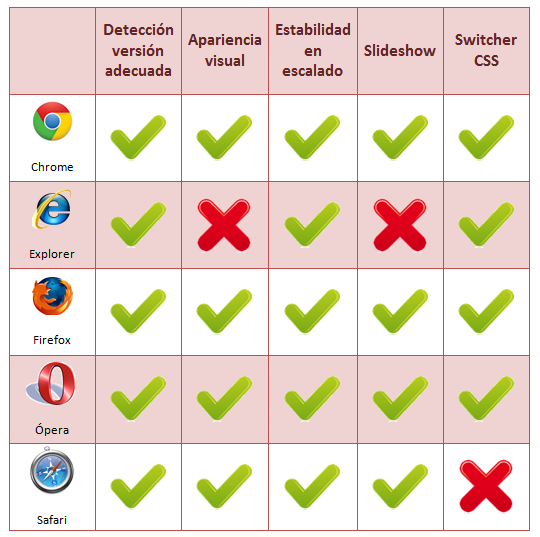
\includegraphics[width=0.6\textwidth]{comparativa.png}
\captionsetup{font={footnotesize,it}}
\caption*{Nota: Para la comparación solamente se comprobó el buen funcionamiento del HTML, CSS y JQuery. (Fuente: \textcite{cobo_2011})}
\end{table}

A continuación se muestra el entorno de trabajo que debes utilizar para citar las tablas:

\begin{lstlisting}[frame=single, float=ht]
\begin{table}[H]
\caption{Titulo de la tabla}
\label{nombre_etiqueta}
\centering
- Aqui va la tabla -
\captionsetup{font={footnotesize,it}}
\caption*{Nota: Informacion referente a la tabla. (Fuente: \textcite{Bibtexkey})}
\end{table}
\end{lstlisting}

Para el caso de una imagen, figura o fotografía, solamente debes colocar la fuente al final del título, como se muestra en el ejemplo de la Figura \ref{escudo}. \textcolor{red}{Cabe señalar que cuando los autores de las fuentes son instituciones, empresas o coporaciones, debes colocar el nombre de la misma entre \{ \} en el campo author de la entrada Bibtex}.

\begin{figure}[H]
\centering

\includegraphics[width=0.3\textwidth]{UC.png} 
\rule{35em}{0.5pt}
\caption{Escudo de la Universidad de Carabobo. \textit{(Fuente: \textcite{UC2015})}}
\label{escudo}
\end{figure}

Para citar la fuente de imágenes puedes utilizar el siguiente entorno:

\begin{lstlisting}[frame=single, float=ht]
\begin{figure}[H]
\centering
\includegraphics{archivo} 
\rule{35em}{0.5pt}
\caption{Titulo de la figura. \textit{(Fuente: \textcite{Bibtexkey})}}
\label{nombre_etiqueta}
\end{figure}
\end{lstlisting}

Cabe señalar que el re-escribir una tabla, o agregarle un poco de información no la convierte en información de tu autoría, lo mismo pasa con aquellas imágenes que por algún motivo debes rehacer de alguna fuente. En estos casos, aunque tu elaboraste dichas tablas o figuras no te hacer el autor original de las mismas, por lo que debes citar dichas fuentes como se muestra en la Tabla \ref{paises}.

Se puede observar de la Tabla \ref{paises}, que aún cuando se tradujo la información y se elaboró la tabla, esta no es de nuestra autoría, por lo que se debe colocar la palabra <<Adaptado de>> antes de citar la fuente. De esta manera se entiende que la tabla, la figura o código mostrado se rehízo por alguna circunstancia y que la idea original proviene de esa fuente citada. Este mismo tratamiento debe realizarse para las figuras.

\begin{table}[H]
\caption{Países o zonas que comienzan por la letra A en inglés}
\label{paises}
\centering
\begin{tabular}{ |p{3.5cm}|p{2.5cm}|p{2.5cm}|p{2.5cm}|  }
 \hline
 \multicolumn{4}{|c|}{Lista de países} \\
 \hline
 Nombre del país o zona & ALPHA ISO  2  & ISO ALPHA 3 & ISO numérico\\
 \hline
 Afganistán   & AF    &AFG&   004\\
 Islas Aland&   AX  & ALA   &248\\
 Albania &AL & ALB&  008\\
 Argelia   &DZ & DZA&  012\\
 Samoa Americana&   AS  & ASM&016\\
 Andorra& AD  & AND   &020\\
 Angola& AO  & AGO&024\\
 \hline
\end{tabular}
\captionsetup{font={footnotesize,it}}
\caption*{Nota: Solo se tomaron los primeros 7 países. Adaptado de (Fuente: \textcite{tables})}
\end{table}

\noindent\textbf{Notas importantes al momento de citar}:

\begin{itemize}
\item No debes citar aquella información que puede encontrarse en muchas fuentes. (Ej: Simón Bolívar murió el 17 de diciembre de 1830 en Santa Marta, Colombia)
\item No debes citar aquello que es fácilmente observable. (Ej: Muchas personas manejan en estado de ebriedad)
\item No debes citar refranes o dichos comunes. (Ej: Cuando el río suena es porque piedras trae)
\end{itemize}
 % Este capítulo contiene toda la información para generar el instructivo. - CUANDO REALICE EL PROYECTO DESACTIVE (COMENTE) ESTA LÍNEA DE COMANDO Y ACTIVE LOS COMANDO CORRESPONDIENTES A CADA CAPÍTULO-.

% Capítulo 1

\chapter{El problema} % Título Principal del Capítulo

\label{Capitulo1} % Para hacer referenciar este capítudo use \ref{Capitulo1}

%----------------------------------------------------------------------------------------
%	SECTION 1
%----------------------------------------------------------------------------------------

\section{PLANTEAMIENTO DEL PROBLEMA}

Lorem ipsum dolor sit amet, consectetur adipiscing elit. Aliquam ultricies lacinia euismod. Nam tempus risus in dolor rhoncus in interdum enim tincidunt. Donec vel nunc neque. In condimentum ullamcorper quam non consequat. Fusce sagittis tempor feugiat. Fusce magna erat, molestie eu convallis ut, tempus sed arcu. Quisque molestie, ante a tincidunt ullamcorper, sapien enim dignissim lacus, in semper nibh erat lobortis purus. Integer dapibus ligula ac risus convallis pellentesque.

%----------------------------------------------------------------------------------------
%	SECTION 2
%----------------------------------------------------------------------------------------

\section{JUSTIFICACIÓN DE LA INVESTIGACIÓN}

Sed ullamcorper quam eu nisl interdum at interdum enim egestas. Aliquam placerat justo sed lectus lobortis ut porta nisl porttitor. Vestibulum mi dolor, lacinia molestie gravida at, tempus vitae ligula. Donec eget quam sapien, in viverra eros. Donec pellentesque justo a massa fringilla non vestibulum metus vestibulum. Vestibulum in orci quis felis tempor lacinia. Vivamus ornare ultrices facilisis. Ut hendrerit volutpat vulputate. Morbi condimentum venenatis augue, id porta ipsum vulputate in. Curabitur luctus tempus justo. Vestibulum risus lectus, adipiscing nec condimentum quis, condimentum nec nisl. Aliquam dictum sagittis velit sed iaculis. Morbi tristique augue sit amet nulla pulvinar id facilisis ligula mollis. Nam elit libero, tincidunt ut aliquam at, molestie in quam. Aenean rhoncus vehicula hendrerit.

%----------------------------------------------------------------------------------------
%	SECTION 3
%---------------------------------------------------------------------------------------

\section{OBJETIVOS}

Sed ullamcorper quam eu nisl interdum at interdum enim egestas. Aliquam placerat justo sed lectus lobortis ut porta nisl porttitor. Vestibulum mi dolor, lacinia molestie gravida at, tempus vitae ligula. Donec eget quam sapien, in viverra eros. Donec pellentesque justo a massa fringilla non vestibulum metus vestibulum. Vestibulum in orci quis felis tempor lacinia. Vivamus ornare ultrices facilisis. Ut hendrerit volutpat vulputate. Morbi condimentum venenatis augue, id porta ipsum vulputate in. Curabitur luctus tempus justo. Vestibulum risus lectus, adipiscing nec condimentum quis, condimentum nec nisl. Aliquam dictum sagittis velit sed iaculis. Morbi tristique augue sit amet nulla pulvinar id facilisis ligula mollis. Nam elit libero, tincidunt ut aliquam at, molestie in quam. Aenean rhoncus vehicula hendrerit.

\subsection{Objetivo General}

\subsection{Objetivos Específicos}

%----------------------------------------------------------------------------------------
%	SECTION 4
%---------------------------------------------------------------------------------------

\section{ALCANCE} % El problema

%% Capítulo 2

\chapter{Marco Conceptual} % Título Principal del Capítulo

\label{Capitulo2} % Para hacer referenciar este capítudo use \ref{Capitulo2}

%----------------------------------------------------------------------------------------
%	SECTION 1
%----------------------------------------------------------------------------------------

\section{Main Section 1}

Lorem ipsum dolor sit amet, consectetur adipiscing elit. Aliquam ultricies lacinia euismod. Nam tempus risus in dolor rhoncus in interdum enim tincidunt. Donec vel nunc neque. In condimentum ullamcorper quam non consequat. Fusce sagittis tempor feugiat. Fusce magna erat, molestie eu convallis ut, tempus sed arcu. Quisque molestie, ante a tincidunt ullamcorper, sapien enim dignissim lacus, in semper nibh erat lobortis purus. Integer dapibus ligula ac risus convallis pellentesque.

%-----------------------------------
%	SUBSECTION 1
%-----------------------------------
\subsection{Subsection 1}

Nunc posuere quam at lectus tristique eu ultrices augue venenatis. Vestibulum ante ipsum primis in faucibus orci luctus et ultrices posuere cubilia Curae; Aliquam erat volutpat. Vivamus sodales tortor eget quam adipiscing in vulputate ante ullamcorper. Sed eros ante, lacinia et sollicitudin et, aliquam sit amet augue. In hac habitasse platea dictumst.

%-----------------------------------
%	SUBSECTION 2
%-----------------------------------

\subsection{Subsection 2}
Morbi rutrum odio eget arcu adipiscing sodales. Aenean et purus a est pulvinar pellentesque. Cras in elit neque, quis varius elit. Phasellus fringilla, nibh eu tempus venenatis, dolor elit posuere quam, quis adipiscing urna leo nec orci. Sed nec nulla auctor odio aliquet consequat. Ut nec nulla in ante ullamcorper aliquam at sed dolor. Phasellus fermentum magna in augue gravida cursus. Cras sed pretium lorem. Pellentesque eget ornare odio. Proin accumsan, massa viverra cursus pharetra, ipsum nisi lobortis velit, a malesuada dolor lorem eu neque.

%----------------------------------------------------------------------------------------
%	SECTION 2
%----------------------------------------------------------------------------------------

\section{Main Section 2}

Sed ullamcorper quam eu nisl interdum at interdum enim egestas. Aliquam placerat justo sed lectus lobortis ut porta nisl porttitor. Vestibulum mi dolor, lacinia molestie gravida at, tempus vitae ligula. Donec eget quam sapien, in viverra eros. Donec pellentesque justo a massa fringilla non vestibulum metus vestibulum. Vestibulum in orci quis felis tempor lacinia. Vivamus ornare ultrices facilisis. Ut hendrerit volutpat vulputate. Morbi condimentum venenatis augue, id porta ipsum vulputate in. Curabitur luctus tempus justo. Vestibulum risus lectus, adipiscing nec condimentum quis, condimentum nec nisl. Aliquam dictum sagittis velit sed iaculis. Morbi tristique augue sit amet nulla pulvinar id facilisis ligula mollis. Nam elit libero, tincidunt ut aliquam at, molestie in quam. Aenean rhoncus vehicula hendrerit. % Marco Conceptual
 
%% Capítulo 3

\chapter{Procedimiento Metodológico} % Título Principal del Capítulo

\label{Capitulo3} % Para hacer referenciar este capítudo use \ref{Capitulo3}

%----------------------------------------------------------------------------------------
%	SECTION 1
%----------------------------------------------------------------------------------------

\section{Main Section 1}

Lorem ipsum dolor sit amet, consectetur adipiscing elit. Aliquam ultricies lacinia euismod. Nam tempus risus in dolor rhoncus in interdum enim tincidunt. Donec vel nunc neque. In condimentum ullamcorper quam non consequat. Fusce sagittis tempor feugiat. Fusce magna erat, molestie eu convallis ut, tempus sed arcu. Quisque molestie, ante a tincidunt ullamcorper, sapien enim dignissim lacus, in semper nibh erat lobortis purus. Integer dapibus ligula ac risus convallis pellentesque.

%-----------------------------------
%	SUBSECTION 1
%-----------------------------------
\subsection{Subsection 1}

Nunc posuere quam at lectus tristique eu ultrices augue venenatis. Vestibulum ante ipsum primis in faucibus orci luctus et ultrices posuere cubilia Curae; Aliquam erat volutpat. Vivamus sodales tortor eget quam adipiscing in vulputate ante ullamcorper. Sed eros ante, lacinia et sollicitudin et, aliquam sit amet augue. In hac habitasse platea dictumst.

%-----------------------------------
%	SUBSECTION 2
%-----------------------------------

\subsection{Subsection 2}
Morbi rutrum odio eget arcu adipiscing sodales. Aenean et purus a est pulvinar pellentesque. Cras in elit neque, quis varius elit. Phasellus fringilla, nibh eu tempus venenatis, dolor elit posuere quam, quis adipiscing urna leo nec orci. Sed nec nulla auctor odio aliquet consequat. Ut nec nulla in ante ullamcorper aliquam at sed dolor. Phasellus fermentum magna in augue gravida cursus. Cras sed pretium lorem. Pellentesque eget ornare odio. Proin accumsan, massa viverra cursus pharetra, ipsum nisi lobortis velit, a malesuada dolor lorem eu neque.

%----------------------------------------------------------------------------------------
%	SECTION 2
%----------------------------------------------------------------------------------------

\section{Cronograma de Actividades}

\begin{figure}
\centering
%------------------------------------------------
%Definiciones Básicas (NO MODIFICAR)
%------------------------------------------------

\definecolor{barblue}{RGB}{153,204,254}
\definecolor{groupblue}{RGB}{51,102,254}
\definecolor{linkred}{RGB}{165,0,33}
%\renewcommand\sfdefault{phv}
\setganttlinklabel{s-s}{Inicio-Inicio}
\setganttlinklabel{f-s}{Inicio-Final}
\setganttlinklabel{f-f}{Final-Final}
\sffamily
\begin{ganttchart}[
%------------------------------------------------
%Encabezado de diagrama (NO MODIFICAR)
%------------------------------------------------
canvas/.append style={fill=none, draw=black!5, line width=.75pt},
hgrid style/.style={draw=black!5, line width=.75pt},
vgrid={*1{draw=black!5, line width=.75pt}},
today=7,  % En este comando se indica el mes en el que se entrega el Proyecto. En caso de que ninguna actividad haya comenzado en el momento de la entrega, desactive (comente) esta línea.  
today rule/.style={
draw=black!64,
dash pattern=on 3.5pt off 4.5pt,
line width=1.5pt
},
today label font=\small\bfseries,
title/.style={draw=none, fill=none},
title label font=\bfseries\footnotesize,
title label node/.append style={below=7pt},
include title in canvas=false,
bar label font=\small\color{black!70},
bar label node/.append style={left=2cm},
bar/.append style={draw=none, fill=black!63},
bar incomplete/.append style={fill=barblue},
bar progress label font=\footnotesize\color{black!70},
group incomplete/.append style={fill=groupblue},
group left shift=0,
group right shift=0,
group height=.5,
group peaks tip position=0,
group label node/.append style={left=.6cm},
group progress label font=\bfseries\small,
link/.style={-latex, line width=1.5pt, linkred},
link label font=\scriptsize\bfseries,
link label node/.append style={below left=-2pt and 0pt}
]{1}{12}
%----------------------------------------------------------
%Fin del Encabezado de diagrama
%---------------------------------------------------------
% A partir de esta linea Ud podrá editar las lineas que aparezcan
%comentadas para adaptar el diagrama de gantt a sus requerimientos

\gantttitle[
title label node/.append style={below left=7pt and -3pt}
]{Meses:\quad1}{1}
\gantttitlelist{2,...,12}{1} \\ % Número de meses.
%Si desea mas especificidad en la fecha, modifique el comando anterior.
\ganttgroup[progress=57]{Revisi\'{o}n Te\'{o}rica}{1}{10} \\%Porcentaje
% de completitud del grupo de actividades.
\ganttbar[
progress=75,% Porcentaje de completitud de la actividad
name=WBS1A
]{Actividad A}{1}{8} \\%Coloque acá la primera 1ra actividad a realizar
% y su duración.
\ganttbar[
progress=67,% Porcentaje de completitud de la actividad
name=WBS1B
]{Actividad B}{1}{3} \\%Coloque acá la segunda 2da actividad a realizar
%y su duración.
\ganttbar[
progress=50,% Porcentaje de completitud de la actividad
name=WBS1C
]{Actividad C}{4}{10} \\%Coloque acá la tercera 3ra actividad a realizar
%y su duración.
\ganttbar[
progress=0,% Porcentaje de completitud de la actividad
name=WBS1D
]{Actividad D}{4}{10} \\[grid]%Coloque acá la 4ta actividad actividad a
% realizar y su duración.
\ganttgroup[progress=0]{Implementaci\'{o}n}{4}{10} \\% Porcentaje 
%de completitud del grupo de actividades.
\ganttbar[progress=0]{Actividad E}{4}{5} \\%Coloque acá la 5ta actividad a realizar y su duración.
\ganttbar[progress=0]{Actividad F}{6}{8} \\%Coloque acá la 6ta actividad a a realizar y su duración.
\ganttbar[progress=0]{Actividad G}{9}{10}%Coloque acá la primera 7ma actividad a realizar y su duración.
\ganttlink[link type=s-s]{WBS1A}{WBS1B} % Esto permite enlazar dichas actividades con los conectores inicio-inicio (s-s), final-inicio (f-s) o final-final (f-f)
\ganttlink[link type=f-s]{WBS1B}{WBS1C}
\ganttlink[
link type=f-f,
link label node/.append style=left
]{WBS1C}{WBS1D}
\end{ganttchart}

\caption{Diagrama de Gantt con indicadores y enlaces}
\label{GanttFig}
\end{figure} % Procedimiento Metodológico


%----------------------------------------------------------------------------------------
%	REFERENCIAS BIBLIOGRÁFICAS
%----------------------------------------------------------------------------------------

\printbibliography

%----------------------------------------------------------------------------------------
\end {document}  
